% This is samplepaper.tex, a sample chapter demonstrating the
% LLNCS macro package for Springer Computer Science proceedings;
% Version 2.20 of 2017/10/04
%
\documentclass[runningheads]{llncs}
%
\usepackage{graphicx}
% Used for displaying a sample figure. If possible, figure files should
% be included in EPS format.
%
% If you use the hyperref package, please uncomment the following line
% to display URLs in blue roman font according to Springer's eBook style:
% \renewcommand\UrlFont{\color{blue}\rmfamily}

\begin{document}
%
\title{A guiding Comparison Matrix of Semantic Restful Web APIs enabling Technologies}
%
%\titlerunning{Abbreviated paper title}
% If the paper title is too long for the running head, you can set
% an abbreviated paper title here
%
\author{Antoine Cheron\inst{1}\orcidID{0000-0003-1857-6799} \and
Johann Bourcier\inst{2}\orcidID{1111-2222-3333-4444} \and
Olivier Barais\inst{2}\orcidID{0000-0002-4551-8562} \and
Antoine Michel\inst{1}}
%
\authorrunning{A. Cheron et al.}
% First names are abbreviated in the running head.
% If there are more than two authors, 'et al.' is used.
%
\institute{FABERNOVEL, 46 rue Saint-Lazare F-75010 Paris \email{firstname.lastname@fabernovel.com} \and
Univ Rennes, Inria, CNRS, IRISA 263 Avenue General Leclerc, F-35000 Rennes
\email{firstname.lastname@irisa.fr}\\
\url{https://www.irisa.fr/fr/equipes/diverse}}
%
\maketitle              % typeset the header of the contribution
%
\begin{abstract}
Semantic RESTful APIs combine the power of the REST architectural style, the Semantic Web and Linked Data. They picture a world in which Web APIs are easier to browse and more meaningful for humans while also being machine-interpretable, turning them into platforms that developers and companies can build on. We counted 38 technologies that target building such APIs. As there is no one-size-fits-all technology, they have to be combined. This makes selecting the appropriate set of technologies to a specific context a difficult task for architects and developers. So, how the selection of such a set of technologies can be eased? In this paper we propose a comparison matrix of Semantic RESTful APIs enabling technologies. It is based on the analysis of the differences and commonalities between existing technologies. The matrix also details what features they make possible or impossible. It intends to help developers and architects in making an informed decision on the technologies to use. It also highlights the limitations of state-of-the-art technologies from which open challenges are derived.

\keywords{Semantic Web\and REST\and Web API\and comparison\and Linked Data}
\end{abstract}
%
%
%
\section{Introduction}

Today, RESTful APIs \cite{FieldingThesis} have become the de-facto standard for building web applications. The main reason behind this popularity lies in the appropriate trade-off between the facility to build such applications and the benefits provided by this approach in such an opened large-scale distributed system: evolutivity, scalability and loose-coupling. However, 95\% of Web APIs are not RESTful \cite{10.1007/978-3-319-38791-8_2} as they claim to be.

Until today, no single standard has emerged to design truly RESTful APIs. Consequently, software architects are facing the challenge of selecting the good technology support for designing and implementing these systems. Typically, a software architect has to select the right interface description language, the right  interchange format and the right framework to ease the development of such APIs.

In addition, a new trend has recently emerged to create RESTful APIs that carry their own semantics, they are called Semantic RESTful APIs~\cite{7195633}. It is a vision that proposes to make fully REST-compliant APIs compatible with the Semantic Web ~\cite{TheSemanticWeb} and Linked Data~\cite{LinkedDataPrinciples}. From our experience at XXX\footnote{company name has been removed for double blind review process}, we have found that building such APIs does not require much more effort than truly RESTful systems, whereas it offers great benefits, such as loose-coupling, automated API mash-ups~\cite{benslimane2008services}, machine-interpretability and very powerful querying. 

However, the design of semantic RESTful APIs considerably increases the complexity for the architect to choose the appropriate technology. Indeed, the specific criteria and properties to be taken into account when choosing an IDL, an exchange format and a framework are not explicit. A decision matrix is missing that would allow the architect to understand the consequences of a design decision, i.e. the characteristics and limitations of each approach.
 
In this paper, we propose to fill this gap by providing decision matrix that help architects to choose the technologies that will best meet their needs. The main contributions of this paper are:

\begin{itemize}
    \item three comparison matrix of interchange formats, interface description languages and frameworks that helps choosing appropriate technologies to build Semantic RESTful APIs
    \item a list of features that are missing from state-of-the-art technologies to allow the creation of RESTful semantic APIs
\end{itemize}

Based on these comparison matrix, we draw the outline of a research road-map to ease the adoption of Semantic RESTful APIs in industry.

The remainder of this paper is organized as follows. Section \ref{sec:background} provides the required background on Web API and REST technology. Then section \ref{sec:maturityLevel} describes the reference maturity level to choose the functionality level of the API and its limitation. The two following sections describes our comparison matrix and an illustration example to highlight the benefit of our proposition. Finally section \ref{sec:discussion} discusses the role of the existing frameworks to build REST APIs. 





%This task is very time-consuming and difficult  because there exist no standard and a lot of candidates to it. Moreover, technologies have subtle differences that may have a big impact on the features the resulting system supports. Identifying them requires reading lots of documentation from specifications, technologies' websites or blog articles as no previous paper addresses this issue.

%In recent years, the concept of Semantic RESTful APIs arose. It proposes to make fully REST-compliant APIs Semantic Web \cite{TheSemanticWeb} and Linked Data \cite{LinkedDataPrinciples} compatible. From our experience at FABERNOVEL, we noticed that building such APIs does not require a lot more effort than truly RESTful systems, whereas it offers great benefits, such as loose-coupling, automated API mash-ups, machine-interpretability and very powerful querying.


\section{Background} \label{sec:background}

% JOHANN -> TODO. I merged section 2 and 3 in this file.

% TODO - From reviewer 2 : Most of the background should be already known by readers and can be shortened/omitted. RESTful technologies are of daily use for anyone interested on Web Technologies.

% TODO - From reviewer 2 : Do not spend an entire section on someone's else work. You can introduce the maturity model as part of the background (even omitting the figure), provide appropriate references and discuss its disadvantages.

This section describes the main concepts related to the design and implementation of Semantic Restful Web APIs.

\subsection{REST}

The REST architectural style imposes constraints on the design of a distributed system to guarantee the following properties: extensibility, evolution, loose-coupling and easy browsing~\cite{FieldingThesis}. To achieve this goal, it proposes six constraints: (i) \textit{client-server}, (ii) \textit{stateless}, (iii) \textit{cache}, (iv) \textit{uniform interface}, (v) \textit{layered system} and (vi) \textit{code-on-demand}. The latter is optional. The \textit{uniform interface} constraint is itself defined by four constraints: (i) \textit{unique identification of resources}, (ii) \textit{manipulation of resources through representations}, (iii) \textit{self-descriptive messages} and (iv) \textit{hypermedia as the engine of application state (HATEOAS)}.

\subsection{Semantic Web and Linked Data}

The Semantic Web~\cite{TheSemanticWeb} envisions the Web as an open platform, where information is machine processable and unstructured. This vision allows to create complex queries gathering information on the whole Web, which would otherwise be impossible.  It also allows global knowledge to grow quickly and easily because this global knowledge can be distributed among the different stakeholders. To achieve this goal, the Semantic Web community offers a unique and comprehensive set of technologies, including a data model, query language, framework, database, ontological languages, exchange formats and more.

The principles of Linked Data are an extension of the Semantic Web. They advise using meaningful URIs to name things and including links to other resources to create an interconnected information structure. 

With Linked Data, the Semantic Web is becoming closer to the uniform interface of REST systems since these principles are equivalent: namely (i) \textit{unique identification of resources}, (ii) \textit{manipulation of resources through representations} and (iii) \textit{hypermedia as the engine of application state (HATEOAS)}. 

\subsection{Semantic RESTful services}

Looking closer at how an API can be consumed, combining REST with Semantic Web and Linked Data looks very promising. Indeed, it describes APIs that can change without breaking client applications. These APIs advertise their available state transitions, therefore enabling automatic composition to create high level services \cite{alarcon2015rest}, on which intelligent software agents can automatically discover the suite of operations to realize complex workflows and even make any API compatible with voice assistants. This is achieved by semantically enriching the data and operations of REST systems with Semantic Web ontology technologies and by linking resources to other resources, making browsing easier.

\subsection{Resource Model}

A resource model aims to model REST systems in which resources are the central element. A resource is any kind of named element, e.g. a photo, a spreadsheet or a table. It has representations, e.g. in the form of a JSON document or even a jpg image, and state transitions, which availability depends on the current state of the system. State transitions can be viewed as operations, either on the resource itself or on others. A common transition refers to a reading operation of another resource. This transition creates a link between the two resources. In the rest of this paper, operations on the resource itself are called operations while operations on other resources are called links.

It is important to note that, the notion of resources cannot be mapped to the notion of class or entity in an object model. Indeed, the distinction between the notion of class and role does not necessarily exist in a resource-oriented approach. As an illustration, \emph{Users} is a different type of resource than \emph{User}.

%as opposed to classes in object-oriented modeling, a collection of resources of type T is another kind of resource than T. As an illustration, \emph{Users} is a different type of resource than \emph{User}.

A resource type behavior may be described with a state machine, as presented in \cite{Schreier:2011:MRA:1967428.1967434}. If a resource's state change, the resource stays of the same type, even if the implementation represents different states with different classes. Each state may have some operations only available in the given state, and others available in every states. Operations have guards, computed from the values of the resource properties and the context, for example the currently connected user.

Everything can be modeled as resources, including descriptions of operations that could then be used to generate actual HTTP operations at runtime. This way, the number of concepts is lowered and the model contain its own description, which leads to systems where the data and their descriptions can be accessed through a single mechanism.

\section{Selecting an API functionality level}\label{sec:maturityLevel}

The first step an architect faces when designing a Web API is to select the features to support.
Architects use a maturity model to help them decide on the supported features. In general, a maturity model is a scale that represents to what level a technology complies with a given architecture. To reach a level, a technology must meet each constraint of the previous levels and of the targeted level.
Currently, the most used maturity model in industry is the Richardson Maturity Model \cite{RichardsonMaturityModel}, which targets building REST APIs. However, we recommend using the WS3 maturity model \cite{7195633} as it extends the Richardson one, and SoHA \cite{SoHA}, with Semantic REST API-enabling constraints.

\subsection{The WS3 maturity model}

In \cite{7195633}, authors describe the WS3 maturity model for classifying Semantic REST Web APIs. WS3 aims at promoting the adherence to REST architectural principles and the adoption of Semantic Web technology to improve the design, reuse, integration and documentation of Web APIs. It classifies APIs along three independent dimensions: \textit{design}, \textit{profile} and \textit{semantic}, as shown in Fig. \ref{WS3}.

\begin{figure}[ht]
  \caption{WS3 Maturity Model (from \cite{7195633})}
  \centering
  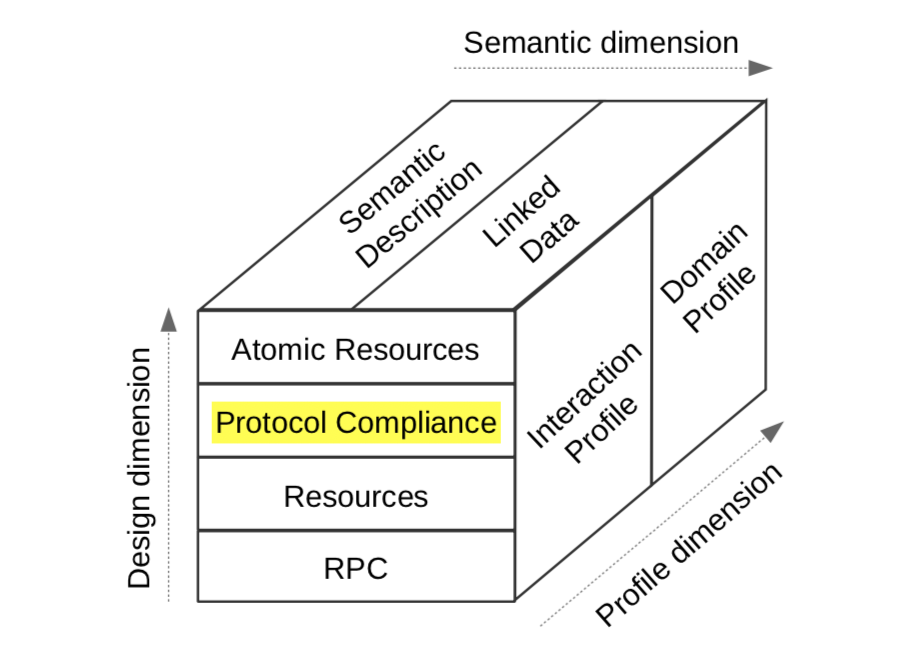
\includegraphics[width=0.47\textwidth]{figures/ws3-maturity-model.png}
  \label{WS3}
\end{figure}

The design dimension represents the different modeling strategies adopted for designing the technical access to a Web API through four levels. The first three levels are similar to the first three levels of the Richardson maturity model. The four levels are (i) RPC-like, (ii) resources have dedicated URI and the API is stateless, (iii) operations on a resource are mapped to HTTP verbs in compliance with the protocol and (iv) the smallest data unit that can be handled by operations is the resource.

The Profile dimension reflects the quality of documentation provided by the Web API through two levels. It takes into account only documentations that can be interpreted by software agents. The first level, interaction profile, requires the description of all available HTTP operations and how to trigger them. The second and final level, the domain profile, requires the description of domain specific details such as the order of operation execution, pre- and post-conditions, business constraints, etc. This level may be reached by providing hypermedia controls at runtime.

The Semantic dimension represents the use of semantic technologies through two levels. To reach the Semantic Description level, an API must semantically describe properties and operations of resources. Next level, Linked Data, is reach when the API semantically describes relationships between resources.

\subsection{Usage}

In their paper, Salvadori \emph{et al.} propose to rate systems along each dimension independently, with a score going from 0 to n, n being the number of levels in the dimension.

For example, a non-documented API with no semantic support that reach level 3 of the Richardson Maturity Model will be rated D3-S0-P0. This means that the API reach the Protocol Compliance level of the Domain dimension and no level of both the Semantic and Profile dimensions.

%For another example, we consider building an API that supports HATEOAS and that provides a swagger-like documentation in the messages at runtime. HATEOAS is used to document available state transitions and to advertise users of the next operations to trigger in order to complete a given business process. This API is rated D3-S0-P2.

A system that supports HATEOAS and provides a swagger-like documentation along with the data, to inform the user of available state transitions, and of the operations to trigger to complete a given business process, is rated D3-S0-P2.

\subsection{Discussion}

The WS3 maturity model is today the most complete maturity model to classify web semantic Rest API. Nevertheless, from our experience at XXX, we noticed two limitations to the applicability of the maturity model to a wider audience. These limitations are related to the Atomic Resources level and the abstraction chosen by the authors.

The Atomic resources constraint requires that the smallest data unit that can be handled by operations is the resource. Let us consider an API handling insurance contracts, that is readable and allows updating the postal address, email address and insurance manager, respecting the Atomic Resources constraint.  Two solutions can be considered. The first one is to create one resource, where every properties can be modified at once, which creates the risk that if two users want to modify two different information at the same time, only one may be made. With this solution, the API would have two operations. The second solution is to create four resources: one for the contract, one for the email address, one for the postal address and one for the manager. The API would have seven operations. The best trade-off would be to create one resource with four operations: (i) read, (ii) update email, (iii) update postal address and (iv) update manager. This solution lowers concurrency risks, the complexity for users and developers is in the middle of the two solutions offered by the Atomic Resources constraint and operations have a more meaningful name.

The second limitation relates to the granularity of the maturity levels. Indeed, each level implies more than one feature. This granularity allows for a coarse-grained categorization of systems. However, to precisely differentiate systems based on the features they implement, a deeper study is needed. Given two systems that reach P1, which means they describe all available HTTP operations and how to trigger them, one might also describe its authentication process and errors whereas the second does not. And yet they reach the same maturity level. As a second example, we consider two systems that describe HTTP operations and domain details such as the order of operations and the authentication process. One might support hypermedia controls whereas the other one has an OpenApi documentation. These two features allow to reach the same maturity level: P2, even though they make a big difference from the client point of view.

\section{Comparison Matrix}\label{sec:matrix}

% ANTOINE -> TODO

% TODO - From reviewer 1 : Section 4.1: The section present a way to select papers, but it is not clear how to select papers concretely. The last three paragraphs in Section 4.1 should be expanded.

In this paper, we propose a fine grain analysis of the API functionality level and a set of comparison matrix to assist the architect in his task of selecting the right technology to build his system. 
Today, there is no single technology to manage all the requested features. Among available technologies, we distinguished three categories:

\begin{itemize}
    \item Interface Description Language (IDL): provide a vocabulary to document domain, functional and non-functional aspects of the API;
    \item Data-Interchange Formats: provide a data-structure, a vocabulary and a layout to share a textual representation of a resource to a user, including its meta-data such as profiles and semantic;
    \item Implementation Frameworks: guide developers in the implementation of the system.
\end{itemize}

In this section we present one comparison matrix per category. Each matrix classifies technologies along the eight levels of the WS3 maturity model, and a fourth category called "other" that contains extra criteria to highlight differences between listed technologies which are not included in the WS3 maturity model. As we showed in the previous section, the WS3 classification is too coarse-grained to grasp all important differences between systems of the same maturity level. Therefore, we present a set of precise criteria for each level to highlight these differences.

\subsection{Comparison Matrix Design Methodology}

% TODO - From reviewer 2 : My impression is that the paper only accounts the result of the web search, and developers' expertise is not actually leveraged. Which are the daily problems developers face? Go deeper with their experience. The framework is intended to be used by developers, you should take into account their insights from the trenches. Interview people from your company if needed, and provide links to their responses/questionnaires.

% TODO - From reviewer 2 : In the same direction, shouldn't popularity be a possible, cross-cutting criteria for comparison? if I choose technology X I'd expect to have a vibrant community to help me with any problem that may arise.

% TODO - From reviewer 2 : The methodology steps can be shortened, as they do not add any useful information. How did you verified the criteria (step v) w.r.t. your previous projects? Provide an example.

% TODO - From reviewer 2 : I cannot stand the number of acronyms the paper introduces. I acknowledge that it's difficult to present big names on tables but this is impossible to follow. E.g., You could numerate or codify approaches (most of them already have a short name) and put them as columns (criteria as rows).

The design of the comparison matrix follows a 5 steps sequential process: (i) looking for candidate technologies, (ii) selecting candidate technology, (iii) deep reading and understanding of each candidate technology, (iv) elaboration of fine grain criteria to characterized and differentiate technologies, (v) verification that the elaborated criteria suited all technologies and the need from XXX developers, and finally (vi) verification that the elaborated criteria highlighted the differences between technologies.

The research of candidate technology (step i) was done through the following steps:

\begin{enumerate}
    \item Identification of the technologies to document APIs. Methods: (i) searching Google and Google Scholar for "service description", "web service description", "web API description", "semantic web service description", "interface description language", "restful service description", "rest API documentation", "rest modeling", "web service modeling" (ii) searching for tools automating tasks from services description, using keywords: "matchmakers", "service composition", "service discovery", "rest service analysis" and (iii) reading the thesis Third Generation Web APIs \cite{lanthalerthird} and \cite{scherer2016description}.
    %Lanthaler:2013:CGW:2487788.2487799
    \item Identification of the technologies to exchange textual documents representing data across distributed systems. Method: (i) searching Google and Google Scholar for: "hypermedia document", "hypermedia format", "RDF format", "RDF document", "data-interchange format", "hypermedia media-type", "semantic web media-type".
    \item Identification of the technologies to implement web APIs. Method: searching Google and Google Scholar for "hateoas framework", "hypermedia framework", "semantic restful framework", "semantic web framework", "linked data framework", "rest API framework", "restful service framework".
    \item Identification of tools to ease the selection of a features set for Web APIs. Method: searching Google and Google Scholar for "rest api best practices", "richardson maturity model", "semantic rest maturity model", "hypermedia api maturity model", "web api best practices", "web api/services categorization".
    \item Selecting papers related to building and evaluating Web APIs from the proceedings of the International Conference on Web Engineering and WS-REST.
\end{enumerate}

From these researches, we selected papers (step ii), articles and web pages that were either the description of a technology, a comparison of technologies or a tool leveraging these technologies. We opened our research to technologies from the 1990s to today. 
From the selected papers and articles, we listed the IDLs, data-interchange formats and frameworks still available to use today.
Then, we read the specification of each chosen technology (step iii) and elaborate classification criteria (step iv). All the raw material used to elaborate this classification is available online\footnote{\url{https://anonymous.4open.science/repository/14273e30-d332-446a-b5a0-df91239532ab/}}. 

We then verified (step v) that the classification criteria suited the needs we had on previous projects we made at  XXX\footnote{company name has been removed for double blind review process} for large companies. 

As a final step (step vi), we read the specifications again to validate that the selected criteria highlighted differences and commonalities well, and to verify results.

All criteria are listed in table \ref{criteria}. Only machine-processable descriptions are considered.

\begin{table*}[ht]
\begin{tabular}{ |P{1.5cm}|p{8cm}| } 
 \hline
 \multicolumn{2}{|c|}{\textbf{Design > Resources}} \\
 \hline
 \textbf{MT} & Models/consider available media types \\
 \textbf{MR} & Models resources \\
 \textbf{MRA} & Models resources' attributes \\
 \textbf{SC} & Separates domain model from URI model \\
 \textbf{OTO} & Operations are associated to their own input and output data model \\
 \hline
 \multicolumn{2}{|c|}{\textbf{Design > Protocol Compliance}} \\
 \hline
 \textbf{MRO} & Supports association of HTTP Verbs to operations \\
 \textbf{EXT} & Extensible with custom data-interchange formats \\
 \textbf{CN} & Support content-negotiation \\
 \hline
 \multicolumn{2}{|c|}{\textbf{Design > Atomic Resources}} \\
 \hline
 \textbf{EAR} & Enforces that the full resource is the smallest data-set operations can handle \\
 \hline
 \multicolumn{2}{|c|}{\textbf{Profile > Interaction}} \\
 \hline
 \textbf{DR} & Describes resources' properties \\
 \textbf{OSD} & Describes HTTP operations \\
 \textbf{LT} & Describes templated URIs \\
 \textbf{CR} & Describes available interchange formats for Read Requests \\
 \textbf{CU} & Describes available interchange formats Update Requests \\
 \textbf{CM} & Describes HTTP verb associated to an operation \\
 \textbf{RUN} & Targets runtime information-enriched description \\
 \textbf{PS} & Supports pagination description \\
 \hline
 \multicolumn{2}{|c|}{\textbf{Profile > Domain}} \\
 \hline
 \textbf{HL} & Provides hyperlinks to other resources as meta-data \\
 \textbf{HYP} & Hypermedia controls \\
 \textbf{MC} & Models and describes business constraints on the data model \\
 \textbf{TI} & Support type inheritance \\
 \textbf{LNM} & Links are modeled by the framework, not added manually in request handlers \\
 \textbf{COA} & Describe conditions to denote an operation/link availability, otherwise the model says they are always available \\
 \textbf{CC} & Conditions for operation/link availability use more information than current resource state, such as the application context, or user-provided information \\
 \textbf{AUT} & Model the authentication mechanism \\
 \textbf{RS} & Describe resources' states \\
 \textbf{SLA} & Describe non-functional properties such as Service Level Agreement \\
 \textbf{ERR} & Describe errors \\
 \hline
 \multicolumn{2}{|c|}{\textbf{Semantic > Description}} \\
 \hline
 \textbf{SD} & Semantically describes resources' properties and HTTP operations \\
 \textbf{DC (opt.)} & Support machine-interpretable and deterministic conditions to denote an operation/link availability \\
 \textbf{RDF} & Support the addition of other RDF vocabularies - makes it RDF-compatible \\
 \hline
 \multicolumn{2}{|c|}{\textbf{Semantic > Linked Data}} \\
 \hline
 \textbf{CL} & Support giving human-interpretable semantic meaning to links \\
 \textbf{SCL} & Support giving semantic meaning to links from RDF vocabulary \\
 \hline
 \multicolumn{2}{|c|}{\textbf{Others}} \\
 \hline
 \textbf{JSON} & JSON-based format \\
 \textbf{ECD} & Entity-centric document as opposed to triple-centric \\
 \textbf{NOM} & No modification on the structure compared to an original JSON file, limited to adding more information \\
 \textbf{HF} & Made for human-readability \\
 \textbf{MF} & Made for machine-readability \\
 \textbf{CUR} & Support for Curies \\
 \textbf{PX} & Uses prefix for reserved keywords to avoid name collision \\
 \textbf{SML} & Support several meta-data level \\
 \textbf{ERS} & Transfer the resource's state explicitly \\
 \textbf{TAR} & Operations have a field to indicate which URI the operation targets, allowing to reference them as resources \\
 \textbf{FSM} & Model the system as a FSM \\
 \textbf{RS} & Model resources as FSM, not only the system \\
 \textbf{STA} & Targets static documentation \\
 \textbf{INC} & Documentation can be split into several pieces \\
 \textbf{FF} & File Format \\
 \textbf{PL} & Programming Language \\
 \textbf{LGEN} & Links to other resources hold by the system are generated at runtime, not written as code \\
 \hline
\end{tabular}
\caption{Matrix Comparison Criteria}
\label{criteria}
\end{table*}

\subsection{Interface Description Language}

% TODO - From reviewer 2 : It's impossible to cover all approaches but you should consider including LRA (Linked Rest APIs) - Linked REST APIs: A Middleware for Semantic REST API Integration, D Serrano, E Stroulia, D Lau, T Ng, Web Services (ICWS), 2017 IEEE International Conference on, 138-145
% and check its related work for others.

% TODO - from reviewer 2 : Include a column on the figures summarizing the number of criteria met by each approach.

% TODO - from reviewer 2 : How did you get columns that are not covered by at least one approach? From the protocol (sec 4.1) it seems that you extracted the criteria by analyzing existing technologies, this means, at least one technology offered it.

Interface Description Languages (IDLs) provide a vocabulary to document domain, functional and non-functional aspects of the API. Non-RDF IDLs are tied to a fixed set of file formats. Meta-models describing Web APIs are IDLs not tied to a file format. We also consider meta-models in this section. We identified 16 candidates that are classified according to 32 criteria in Figure \ref{idl-matrix}.

When IDLs and data-interchange formats are both compatible with RDF, they can be combined to form a file format that can be used as both the data-interchange format and the IDL. This has great benefits in terms of complexity and maintainability.

\subsubsection{Proper Meta-Models}

Among the 16 classified IDLs, 4 are meta-models. In \cite{Rapido} authors present a tool to sketch CRUD or Hypermedia APIs. When selecting Hypermedia APIs, users have to choose one media-type, either HAL or Collection+JSON and then start sketching the application using state machines. \cite{Schreier:2011:MRA:1967428.1967434} models each resource type as a finite state machine with deterministic state transitions. In this model, each resource type has a single initial state, operations can go beyond CRUD and conditions can be modeled to inform the availability of operations. However, conditions are not modeled in more details, which does not make them machine-interpretable. Authors propose to add this capability in future work. In \cite{10.1007/978-3-642-22233-7_24}, authors propose to model the whole system as a non-deterministic state machine. This method makes software agents unable to discover the set of messages to exchange in order to make available an operation that is not at the moment the user would like to invoke it. Haupt et al. \cite{10.1109/ICWS.2014.30} propose a very thorough multi-layered model that separates the domain model from the URI model. It does not allow specifying conditions on the availability of operations and see resources as having a static structure, making it impossible to represent different state of a resource with different classes. 

\subsubsection{Meta-Models from Interface Description Languages}

The 11 interface description languages we found are Hydra Core Vocabulary \cite{Lanthaler:2013:CGW:2487788.2487799}, Atom Syndication Format\cite{AtomSF}, WSDL+SAWSDL, WADL, OpenApi (used by Swagger), API Blueprint, hREST + microWSMO, RESTdesc, RADL, RAML and I/O Docs. We decided to include WSDL+SAWSDL even though it targets RPC-like applications over HTTP \cite{john2012framework}, because it tackles the problem of semantically describing HTTP services.

% FIGURE OF THE IDL CLASSIFICATION
\begin{figure*}[t]
\caption{Interface Description Languages Comparison Matrix}
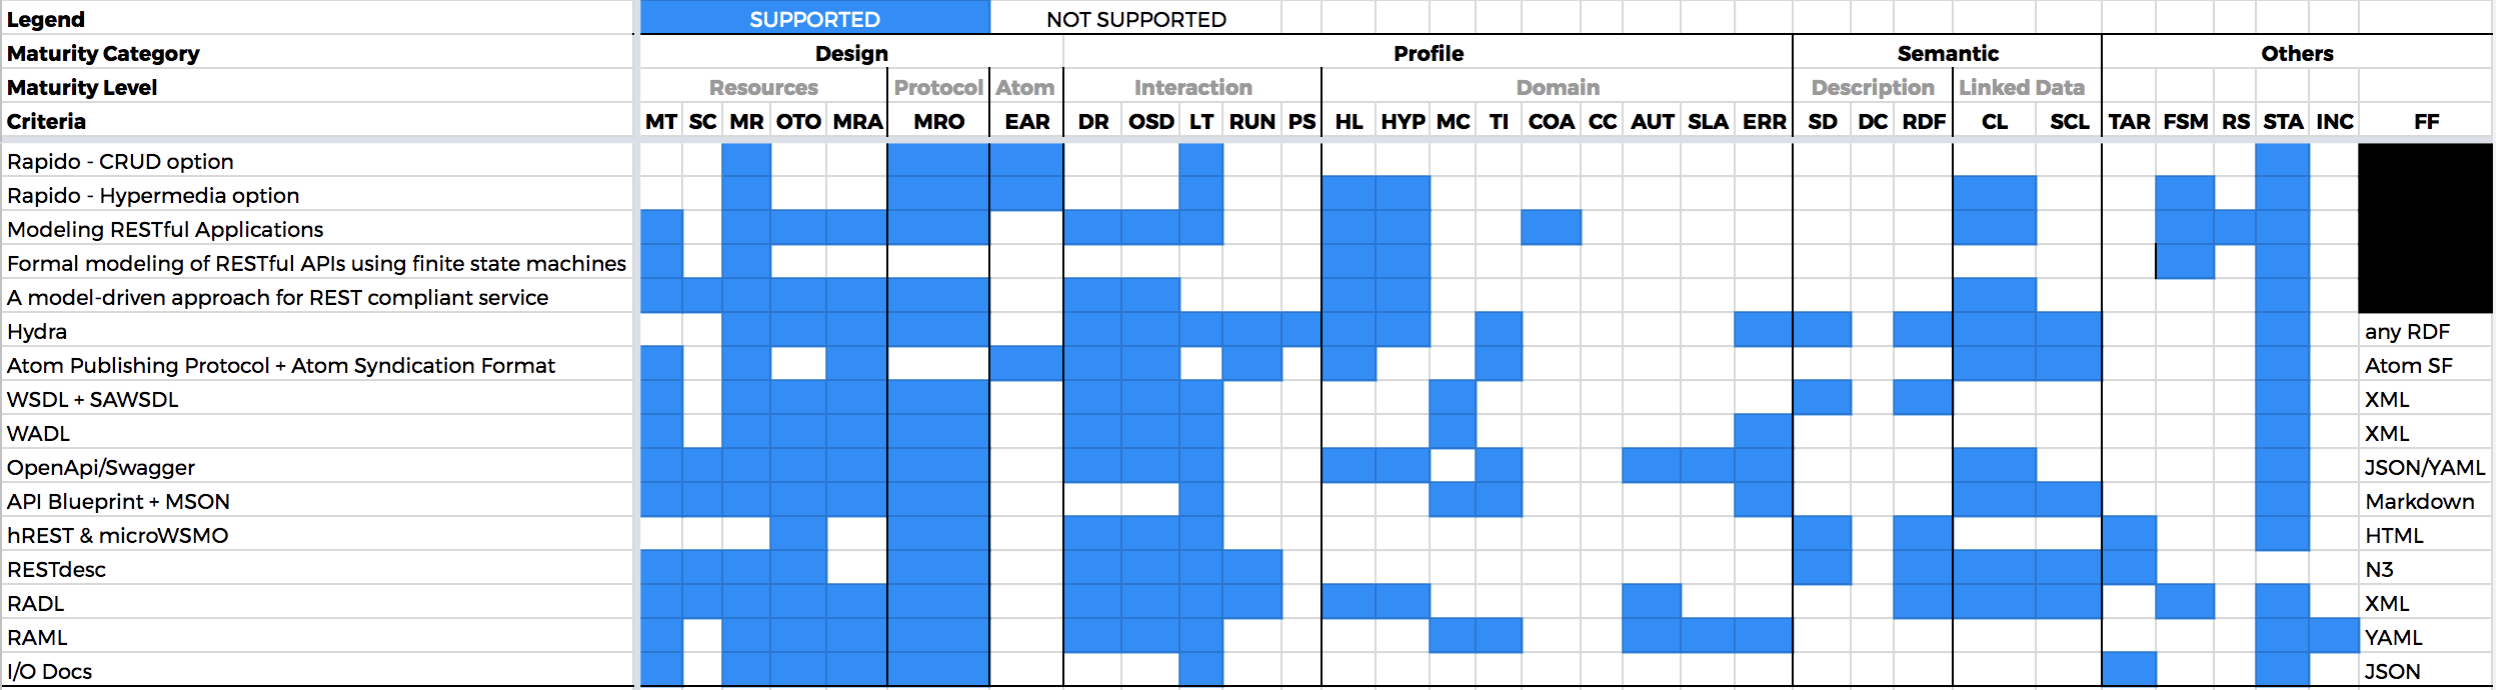
\includegraphics[width=1\textwidth]{figures/IDL.png}
\label{idl-matrix}
\end{figure*}

\subsubsection{Conclusions}

The first thing the matrix highlights is that most IDLs ignore the domain and semantic description of APIs. In addition, they focus on the static documentation of the entire API made for developers, rather than the documentation enriched with information on the current state of the system to guide users when browsing the API.

From this matrix, we observe that Hydra and RESTdesc are the two approaches reaching the highest maturity level. This is because they both semantically describe metadata, use additional RDF vocabularies and target API documentation enriched with execution information.

Only one approach \cite{Schreier:2011:MRA:1967428.1967434} support conditional availability of links between resources and no one makes this meta-data machine-interpretable. This makes software agents unable to find a way to make an operation available when it is not.

Four technologies support the addition of business constraints to the model, and three are machine-processable. We encourage authors of meta-models to add this feature to their technology because it is a step forward in lowering coupling and improving user experience. For example, this allows forms to be automatically generated with client-side data validation.

Finally, this matrix highlights that three out of four scientific publications recommend the modeling of RESTful systems as state machines whereas all except one IDL authors ignore this technique. However, the use of deterministic state machines encourages API designers to think about the domain model in depth. It is then easier to determine if an operation on a resource is not available.

\subsection{Data-interchange formats}

The data-interchange formats can be differentiated based on their compatibility with RDF, which determines if they are extensible. Because they are extensible, RDF formats propose very few features by default. We selected three vocabularies (i) Hydra, (ii) HTTP RDF and (iii) SHACL, an RDF schema validation vocabulary, that we combined with one RDF format, JSON-LD, to show what is possible to do.

When building an API that provides no meta-data, JSON, XML and YAML are the three formats widely used in industry.

On the other side, when the system to build have to send meta-data, no data-interchange formats is considered as a standard today. We found eleven propositions on the web, from scientific publications, GitHub repositories, private web sites, IETF and W3C drafts. They are classified in Fig. \ref{interchange-formats-matrix} according to 26 criteria.

% FIGURE OF THE INTERCHANGE FORMATS CLASSIFICATION
\begin{figure*}[t]
\caption{Data-interchange Formats Comparison Matrix}
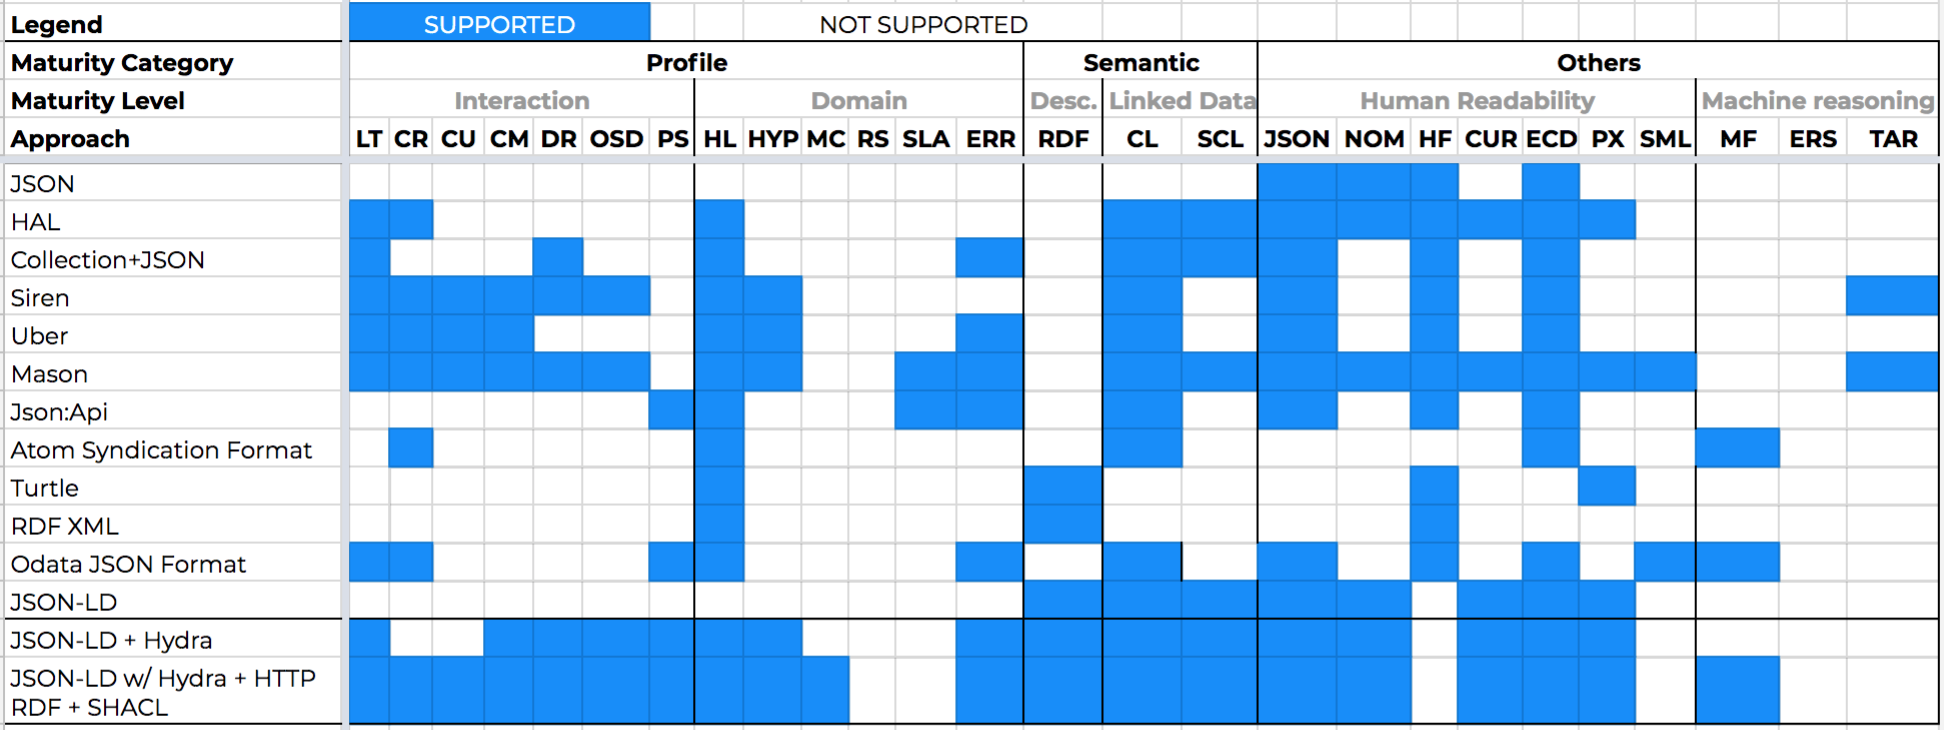
\includegraphics[width=1\textwidth]{figures/DIF.png}
\label{interchange-formats-matrix}
\end{figure*}

\subsubsection*{Conclusions}

On the one hand, non-RDF formats do not allow to reach any level on the semantic axis. However, some of them allow to link the data to others, and to reach the highest level on the \textit{Profile} dimension.
On the other hand, RDF formats can become very expressive when combined with vocabularies. The example with JSON-LD + Hydra + HTTP RDF + SCHACL shows this. However, they require more effort to find appropriate vocabularies on the web.
Furthermore, the matrix highlights that most formats are not readable by machine.

Last, the matrix shows that no format support the description of constraints on the data neither the advertisement of resource's state. Though, most scientific approaches we found describe REST APIs as state machines. Providing the resource's state would ease machine-reasoning. On the other hand, describing the constraints could greatly decrease coupling and increase user experience.

\subsection{Implementation Frameworks}

% TODO - from reviewer 2 : Maybe it's out of scope but I think Loopback (https://loopback.io/) should be analyzed as a framework as it provides/leverages some semantic sugar.

Implementation frameworks are software libraries that guide developers through the implementation of Web APIs. We limit the comparison to frameworks that claim to support HATEOAS. We identified six frameworks that do so.

In \cite{salvadori2014framework} authors propose a Java framework based on JAX-RS 2.0 that uses annotations to semantically describe REST APIs. The end result is a JSON-LD document, enriched with the Hydra vocabulary, that describes the whole API. In \cite{parastatidis2010role} Parastatidis et al. present Restfulie, a framework to ease the development of REST APIs using resources, content-negotiation and state transitions as its core building blocks. Besides these frameworks, we found that API-Platform, Spring HATEOAS, JAX-RS and Ripozo support HATEOAS features. They are classified in Fig. \ref{frameworks-matrix} according to 29 criteria.

% FIGURE OF THE INTERCHANGE FORMATS CLASSIFICATION
\begin{figure*}[t]
\caption{Implementation Frameworks Comparison Matrix}
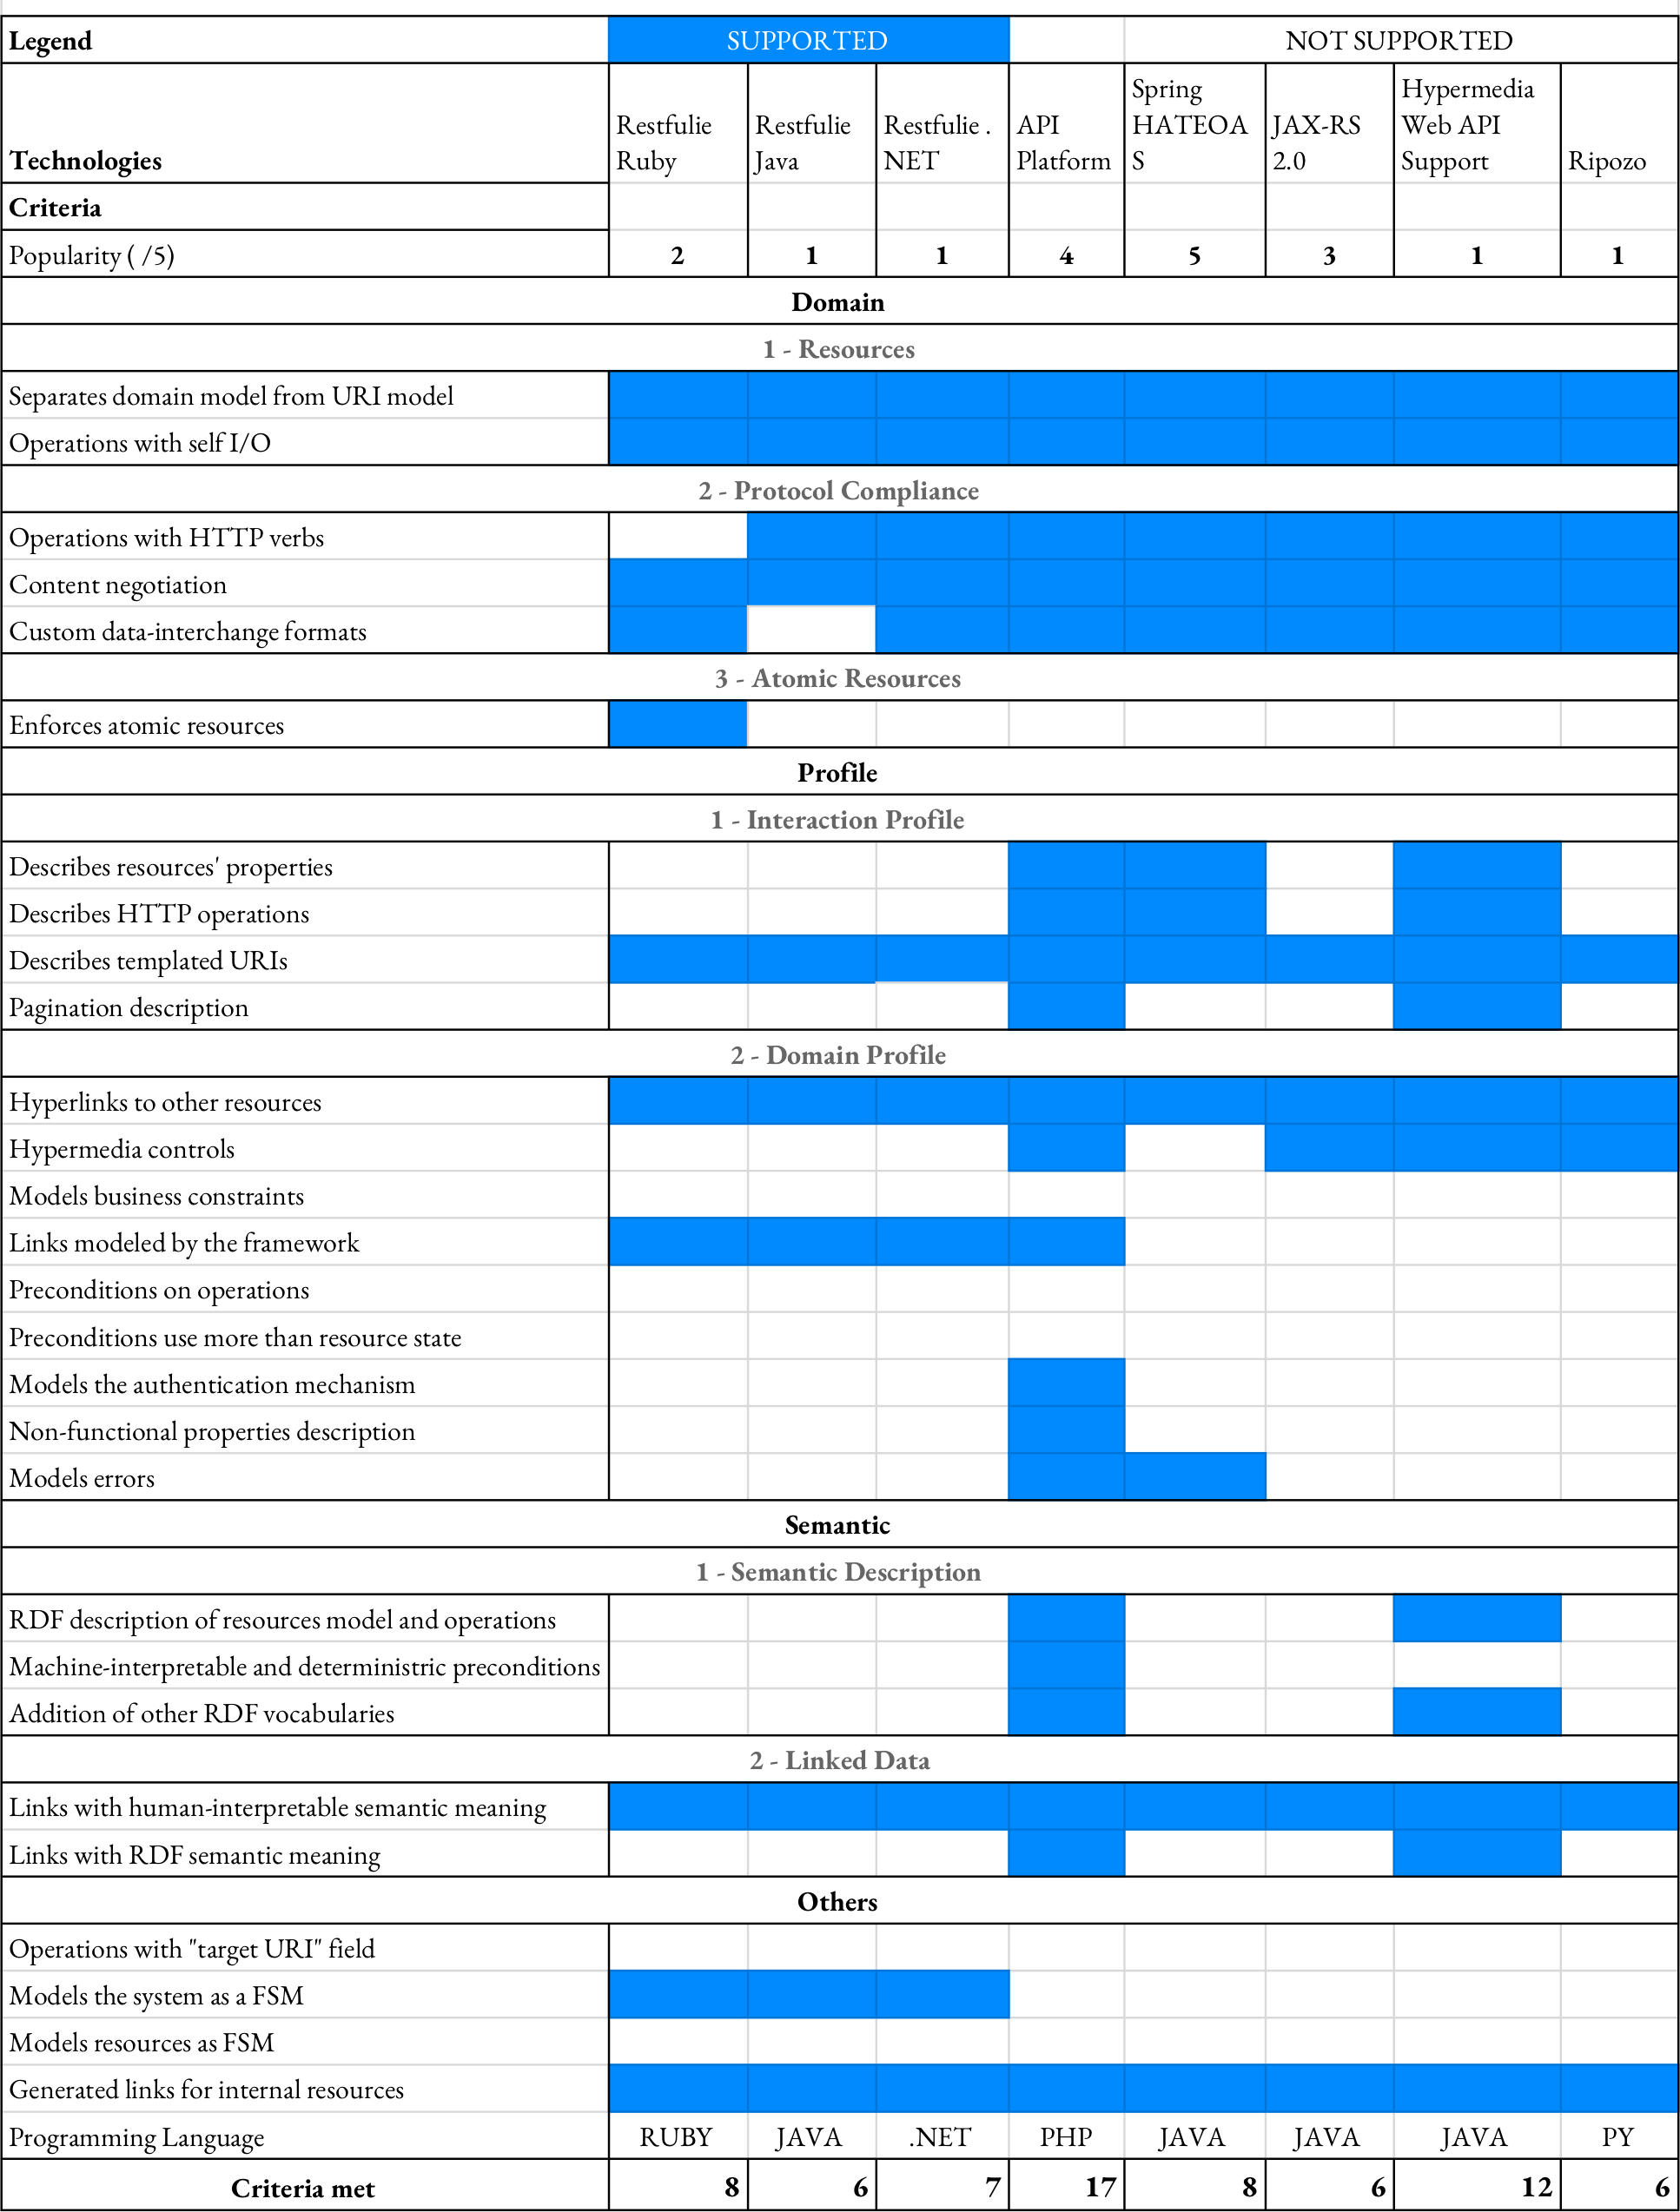
\includegraphics[width=1\textwidth]{figures/frameworks.png}
\label{frameworks-matrix}
\end{figure*}

\subsubsection*{Conclusions}

Despite the fact that only one framework enforces the atomic resources constraint, all frameworks allow to reach the highest level of maturity on the Design axis easily. This is because supporting the Atomic feature is a constraint that can be easily added by the developers themselves. 

We notice that only \textit{APIPlatform} and \textit{Restfulie} support a mechanism to model links instead of adding them programmatically in the resource, thus increasing maintainability.

Otherwise, most framework do not ease the process of documenting and making the API Semantic Web and Linked Data compatible. To us, this is the biggest challenge framework designers are facing today.

As with IDLs, most creators of frameworks do not provide mechanisms to describe resources as state machines even though it could bring the same benefits.

\section{Usage Example}

% ANTOINE -> TODO

% TODO - from reviewer 2 : Case study should be about real systems, not a toy example which suddenly enforces all the maturity restrictions (why such a naive system would be so constrained (maturity D3-S2-P2)?). You could provide insights about a case in your company XXX. Or ask for developer's feedback with real-world systems.

% TODO - from reviewer 2 : Individual figures (Users, Playlists, Songs) take too much space, they can be replaced for a single Table or Figure (Class diagram-esque).

% TODO - from reviewer 2 : How did you define the criteria (a.k.a. the list of unknown acronyms) that the technology for your case study should meet(beginning of Sec. 5.2, 5.3 and 5.4)? those seem to be pulled out from thin air.

This section illustrates the usage of the presented classification matrix to build a system with a targeted maturity level in mind.

\subsection{Example system presentation}

The system we use for this example almost targets the highest maturity of WS3 (D3-S2-P2). Indeed, it does not target to meet the Atomic Resources constraint. It is a music sharing API that allows one to search for songs and playlists. Logged in users can submit songs that will be reviewed by administrators of the platform. If accepted, songs will become publicly available. Songs and playlists have three states: (i) submitted, (ii) accepted or (iii) rejected. Besides that, each user can create up to ten playlists.

Therefore, this API has six types of resources: (i) user, (ii) collection of users, (iii) song, (iv) collection of songs, (v) playlist and (vi) collection of playlists. These types are presented as a resource model in figures 1--3.

Each collection of another type of resource contains a \textit{listAll...(filters)} operation. For the purpose of this paper, we consider that \textit{filters} corresponds to the query parameters of the URI. For example \textit{myapi.com/songs?title=foo\&artist=bar} results in \textit{filters} having a field \textit{title} with value \textit{foo} and another one \textit{artist} with value \textit{bar}. We consider that a collection can be filtered on each property of the resource type it holds. So, \textit{Songs} have \textit{id}, \textit{artist}, \textit{title} and \textit{file} filters.

\begin{figure}[ht]
\caption{Users resource model}
\centering
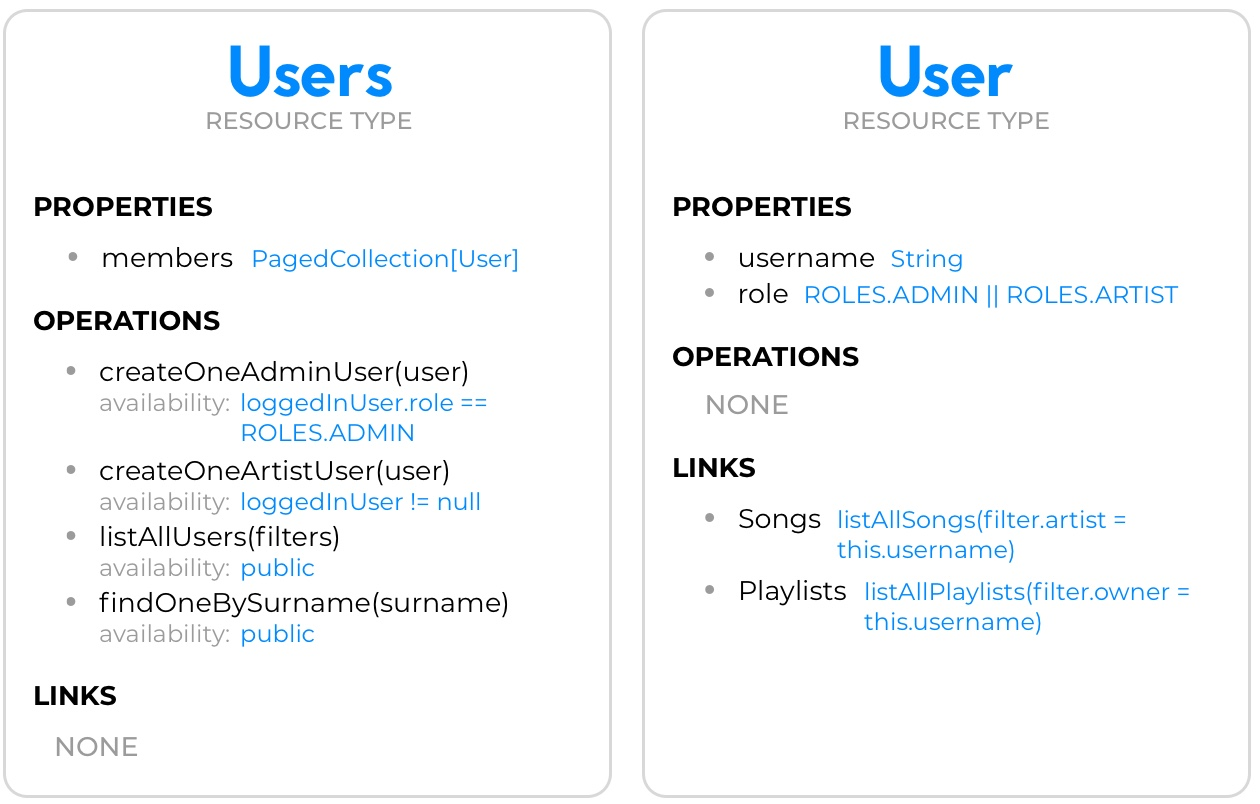
\includegraphics[width=0.47\textwidth]{figures/users.jpg}
\end{figure}

\begin{figure}[ht]
\caption{Playlists resource model}
\centering
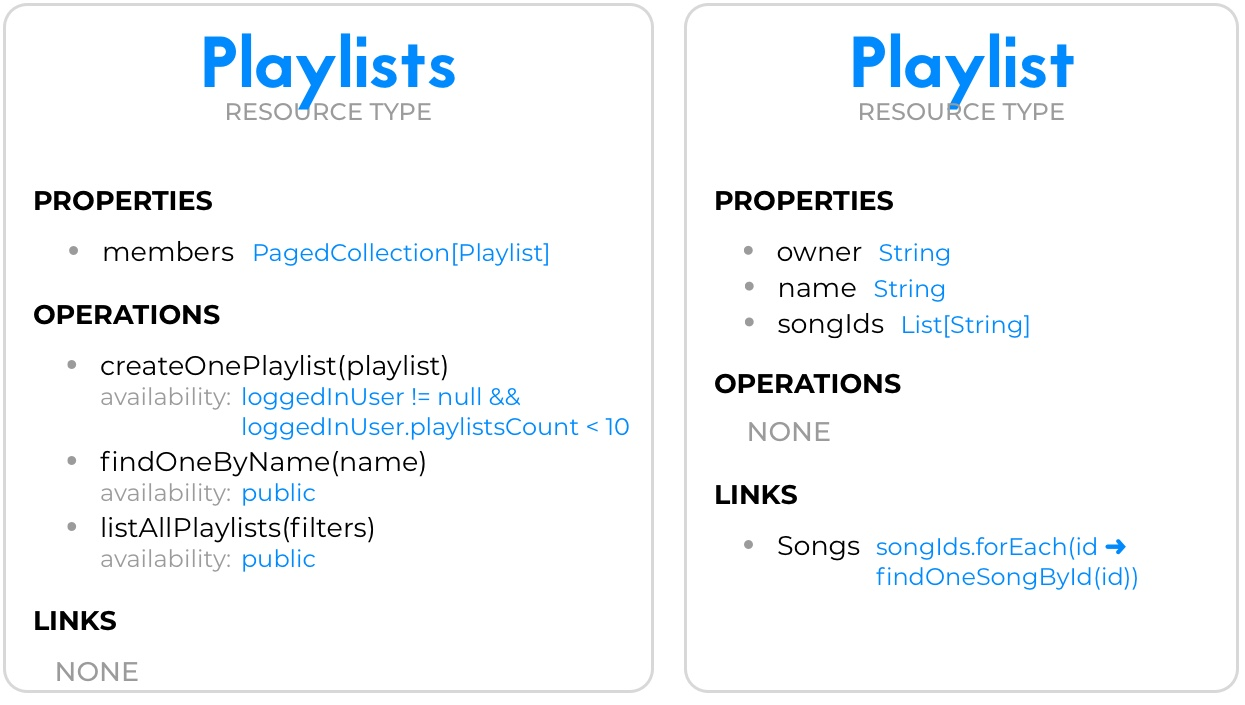
\includegraphics[width=0.44\textwidth]{figures/playlists.jpg}
\end{figure}

\begin{figure}[ht]
\caption{Songs resource model}
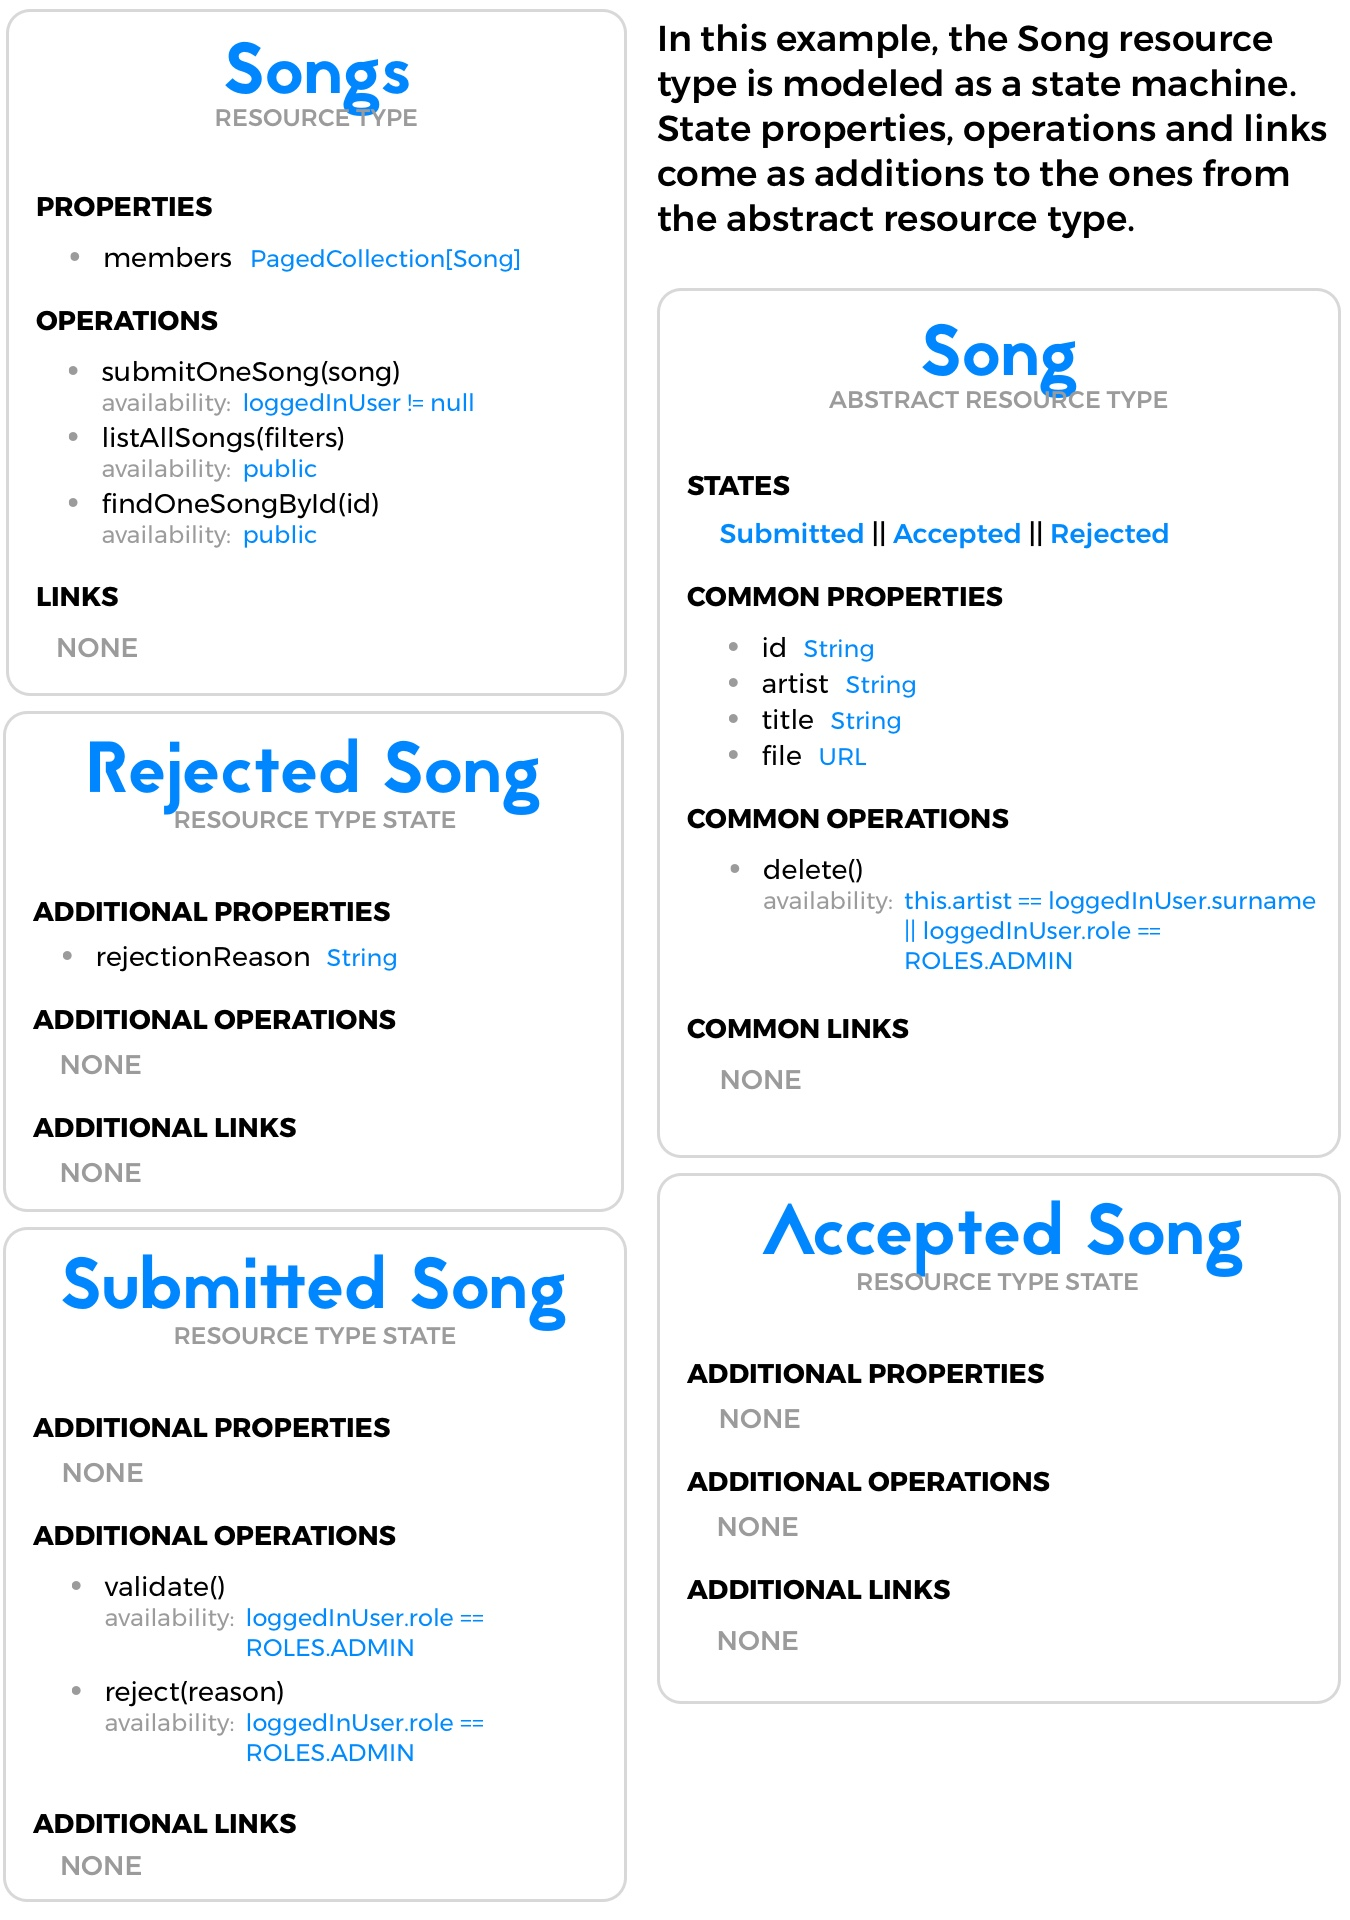
\includegraphics[width=0.44\textwidth]{figures/songs.jpg}
\end{figure}

The domain of this API has four more constraints that are not represented on the resource model. They are:

\begin{itemize}
    \item Calling \textit{Songs.submitOne(song)} as an admin will create an AcceptedSong;
    \item Calling \textit{Songs.submitOne(song)} as an artist will create a SubmittedSong;
    \item A \textit{Playlist.name} can be composed only of characters, spaces and numbers;
    \item A \textit{User.surname} can be composed only of characters, dots and numbers.
\end{itemize}

On the \textit{Profile} aspects, the system should (i) advertise the resource's state explicitly, (ii) provide a documentation of resources and operations, (iii) document its authentication mechanism, (iv) document all information visible in the resource model and (v) support HATEOAS. Each documentation must be machine-processable.

On the \textit{Semantic} aspects, the system should (i) propose an RDF format, to be compatible with the Semantic Web, (ii) link data to others using RDF vocabulary to express relationships and (iii) provide the semantic of the data, their properties and operations.

This system targets humans first, while still requiring machine-interpretability, and must send hypermedia controls through a JSON format. Offering only one interchange format is sufficient.

\subsection{Finding the appropriate Interface Description Language}

To find the most appropriate Interface Description Language to this system, we first need to find the criteria that the technologies we are looking for should meet. In this scenario, they are: \textit{MR, MRA, MRO, OTO, DR, OSD, LT, HL, HYP, MC, COA, CC, AUT, SD, DC, RDF, CL} and \textit{SCL}. The plus are: \textit{SC, RUN, PS} and \textit{RS}. It is a total of 22 criteria.

% TODO - From reviewer 1 : in Section 5.2, the example needs to consider 22 criteria, but there is no justification why the criteria should be considered when implementing the example

The three technologies that meet the highest number of these criteria are: Hydra (15), the model presented in Modeling RESTful Applications \cite{Schreier:2011:MRA:1967428.1967434} (12) and WSDL+SAWSDL (10). In this scenario, the architect would have to make his decision depending on how important and costly to implement are the features that are not supported by the technologies.

% TODO - From reviewer 1 : it is not clear why the three technologies are good because these technologies do not satisfy some criteria

\subsection{Finding the appropriate data-interchange format}

For this category, the criteria technologies should meet are: \textit{LT, CM, OSD, DR, PS, CL, SCL, RDF, JSON, HL, HYP} and \textit{RC}. The plus are: \textit{NOM, HF, PX, ECD} and \textit{CUR}. It is a total of 17 criteria. In addition to meet as much criteria as possible, the interchange format should be compatible with the IDL chosen at the previous step. This is particularly important when an RDF IDL has been chosen as it lowers the number of functionality provided by each technology, making them easier to replace.

The three technologies that meet these criteria best are: Mason, JSON-LD with Hydra, and Siren. JSON-LD is the only one JSON  format designed for RDF, even though others support adding vocabulary. Combined with Hydra they meet 15/17 criteria. Mason meet 15 criteria and Siren 10. This time, selection depends on the chosen IDL, or might influence the IDL choice.

Mason and JSON-LD with Hydra meet the highest number of criteria. Because JSON-LD is the only one RDF format in the list, it makes it a more interesting option. However, each technology leaves non-supported features that the development team will have to implement by itself.

\subsection{Finding the appropriate development framework}

In this scenario, an architect would be looking for a framework that meet the criteria \textit{SC, OTO, MRO, EXT, DR, OSD, LT, PS, HL, HYP, MC, LNM, COA, CC, AUT, ERR, SD, DC, RDF, CL} and \textit{SCL}. If a framework already supports the previously chosen IDL and data-interchange format, it would be a plus and \textit{EXT} would become unnecessary.

From those criteria, the technology that meet the highest number of criteria is API Platform with 18, A framework for semantic description of RESTful APIs comes second with 14 and Spring HATEOAS with 10. In this scenario, an architect would likely opt for API Platform.

\subsection{Results}

% TODO - from reviewer 2 : Section says that "the choice is not straightforward because no technology meet al the criteria" but in the next sentence you just select one for each category! how do you support such decision? which are the particular "context of the project" circumstances that led you to do so? That's why I'd prefer a real case study with real constraints. 

% TODO - from reviewer 2 : Apart from that, a "results" section with only one paragraph and no actual finding does not give that much for the reader and could be removed.

In this section we gave an example showing how to use the proposed classification matrix. Even though the choice is not straightforward because no technology meet all the criteria, it is easy to reduce the number of candidate to three, and then make an informed decision based on the context of the project.
From this scenario, we would have gone with Hydra, JSON-LD and API-platform.

\section{Discussion} \label{sec:discussion}

% ANTOINE -> TODO

% TODO - from reviewer 2 : I agree with the fact that GraphQL is way more adopted than RDF-based semantic approaches, but how does it comes out from your previous analysis? GraphQL was not even mentioned before, and does not arise from the results. Please clarify how can one conclude that, by means of references and evidence from your analysis.

% TODO - from reviewer 2 : Finally, as a future work, authors could automatize the process to help developers in the form of a tool or wizard. -> already in progress

As indicated in the tables proposed in section \ref{sec:matrix} and in the example presented in the previous section, there is no framework yet available to build a semantic REST API. This section discusses, from our perspective, why there is no standard solution to meet all the criteria. These limits also make it possible to initiate research initiatives for the community. 

First, there is no IETF or W3C standard interchange format for building semantic REST APIs. In addition, none of the existing interchange formats support all the criteria described above, nor are they widely adopted, making it likely that new formats will emerge. For this reason, frameworks supporting semantic REST APIs will be forced to rely on formats that are prone to evolve, which will require additional effort and costs. This reduces the likelihood that developers will invest time in developing such features for their framework.

The second reason is that most developers ask for more support for GraphQL and streaming than for Semantic REST. We believe that this is due to two reasons. First of all, GraphQL and streaming are well understood and known, which is unfortunately less the case with RESTful semantic API concepts. Second, there is currently no tool that leverages the power of REST semantic APIs. Thus, being compatible with Semantic REST requires additional efforts to adapt client libraries and to train developers. We believe that with new tools, such as front-end clients, automated test libraries, improved documentation generation and HTTP clients such as Postman, developers would be more interested in semantic REST features.


\section{Conclusion}

In this paper we presented three comparison matrices that help architects choose the Semantic RESTful APIs enabling technologies that meet their needs.
We used an example to show how simple it is to reduce the list of technologies to three when the characteristics to be implemented are identified.
In future work, we plan to make these matrices available online through semantic restful APIs and to improve their accessibility to facilitate technology selection.

We also pointed out that some important features are missing in current technologies. The modeling and description of constraints and conditions indicating the availability of state transitions are ignored by IDL, vocabularies, interchange formats and frameworks. On the other hand, modeling resource as FSM is not available in most frameworks. In addition, IDLs target the documentation of the entire API in a single file. This prevents them from being used for hypermedia controls. Finally, very few tools take advantage of the power of RESTful semantic APIs, and interest around this topic is still low.

Based on these findings, we identify three areas for improvement: (i) adoption, (ii) semantics and documentation, and (iii) implementation. Adoption can be made easier and more beneficial with new tools that leverage the power of these APIs. The discovery and selection of semantic vocabulary should be simplified and the addition of new vocabulary would allow systems to be described more accurately and more thoroughly. This would reduce coupling and increase both composability and navigation.


%
% ---- Bibliography ----
%
% BibTeX users should specify bibliography style 'splncs04'.
% References will then be sorted and formatted in the correct style.
%
% \bibliographystyle{splncs04}
% \bibliography{mybibliography}
%

\bibliographystyle{splncs04}
\bibliography{bibliography}

\end{document}
